\chapter{Introduction}\label{chapter:introduction}
 
The company AGnet has an outdated monolithic system to manage its customers, sales and so on. The technology stack is outdated which is why a migration to a newer technology is necessary. The new architecture should consist of micro-frontends and microservices. Some microservices are already in development, the micro-frontends should be prototyped in the course of this work. Micro-frontends have different problems than traditional frontend-applications. The prototype that is developed should tackle the problems that a distributed architecture brings to the table.
 
This project report is structured in a theoretical part. It is followed by a practical part. In the final chapters the results of the work are presented and discussed. This chapter describes the motivation the hypothesis and state-of-the-art solutions for the project report. Chapter \ref{chapter:applied-methods} covers the methods applied to optimize the number of requests and reduce the network-traffic. The results can be found in Chapter \ref{chapter:results} and the discussion resolving around the result is in Chapter \ref{chapter:discussion}. The final Chapter \ref{chapter:conclusion} concludes the report.

\section{State of the art}

This chapter provides information about state-of-the-art software architecture and integration styles relevant for this project. A short section is dedicated to every relevant technology of this report.

\subsection{Micro Frontends}

Micro-frontends should bring the same advantages of microservices from the backend to the frontend. Instead of creating a large frontend monolith, a micro-frontend architecture contains many small applications. The advantage is that every micro-frontend can be developed and deployed by a separate team. \cite{book:2020:geers:micro-frontends-in-action} The difference between frontend-monoliths and micro-frontends can be seen in figure \ref{figure:state-of-the-art:ui-monotlith-micro-frontend}.

\ifshowImages
\begin{figure}[H]
\centering
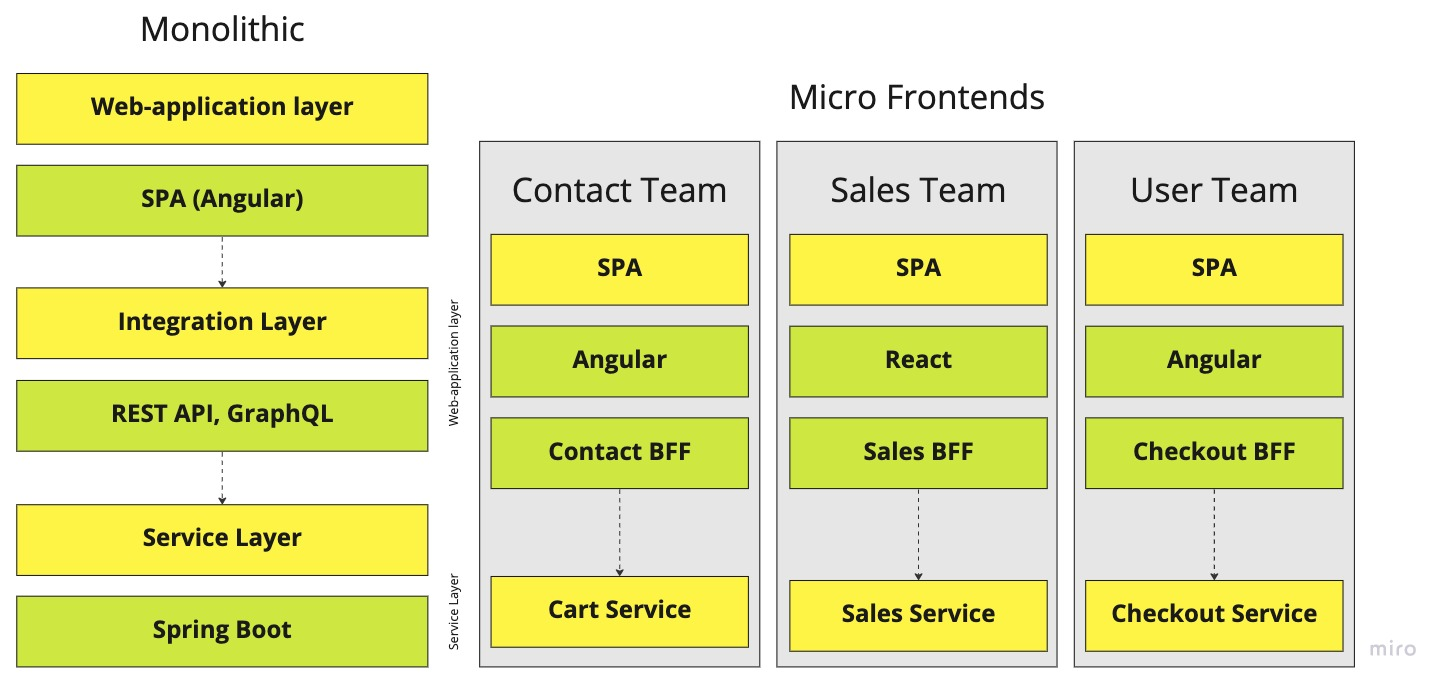
\includegraphics[width=0.8\linewidth]{images/ui-monotlith-micro-frontends.jpg}
\caption{A comparison between frontend-monoliths and micro-frontends.}\label{figure:state-of-the-art:ui-monotlith-micro-frontend}
\end{figure}
\fi


Benefits gained from working with microservices on the backend are lost, when working with a monolithical frontend. With a monolithic frontend, the ability to deploy independently is lost. The entire frontend has to be deployed at once. Another problem is, that distinct operations are not really possible. If one part of the frontend is broken, there is a good chance that the entire frontend is broken. Another problem is the parallel development. The speed of development cannot be increased because it is very difficult to have multiple teams working on one frontend application. \cite{misc:2019:leitner:micro-frontends}

The term micro-frontend can be misleading, as can the term microservice. It has no meaning in terms of the size of the application. It can be a simple widget that only displays data, or a full-blown one-page application. Ideally, a micro frontend covers an area of the entire frontend application.

\ifshowUnusedContent
% TODO(FM): Integration strategy not really important for short explaination
Micro-frontends offer various strategies for integration. Integration means how the frontends are composed on the frontend. The web allows multiple strategies to incorporate the micro-frontends. 

[1] M. Bischof and D. Leitner, “Analysis of the Suitability of a Microservice and a Micro-Frontend Architecture for an Existing Monolithic System,” p. 88.

\begin{itemize}
    \item Server Side Integration 
    \item Client Side Integration
    \item Build time Integration
\end{itemize}

\fi

\subsection{Generic APIs vs Consumer Driven APIs}

The big decision in micro-frontend API development is to use either generic or consumer-oriented APIs. The difference is that generic APIs place great emphasis on reusability, while consumer-oriented APIs tailor the APIs to the customer.

\subsubsection{Generic APIs}

Generic APIs refer to APIs that are very general and can be used by different clients. However, this type of API has two major drawbacks. Over-fetching describes the problem of getting more data than is needed. Over-requesting describes the problem of needing multiple requests to get the data for a use case. Both problems are discussed in more detail in the next paragraphs. \cite{misc:2019:leitner:backend-for-frontends}

\paragraph{Over-Fetching}

For example, a contact service provides a contact-model that includes customer-number, first-name, second-name, uid-number and the address of the user, as seen in listing \ref{code:state-art:over-fetching}. However, one requirement of the application is to display only a contact's first and last name inside the header. Only two fields of the model are used, and the rest are unnecessarily queried. \cite{misc:2019:leitner:backend-for-frontends}

\ifshowListings
\begin{listing}[H]
\begin{minted}{typescript}
interface ContactModel {
  id: string;
  customerNumber: string;
  firstName: string;
  secondName: string;
  uidNumber: string;

  Address: {
    id: string;
    postalCode: string;
    location: string;
    Country: string;
  }
}
\end{minted}
\caption{Contact-Model that contains too much fields for the requirement.}\label{code:state-art:over-fetching}
\end{listing}
\fi

\paragraph{Over-Requesting}

Attempting to solve the problem of over-fetching by reducing the amount of data set that is returned leads directly to this problem. Listing \ref{code:state-art:over-requesting} shows the problem of over-requesting. If another requirement inside the application should display the address alongside the contact, two requests have to be performed every time. Afterwards, the two data sets have to be merged, which leads to high complexity on the client side. \cite{misc:2019:leitner:backend-for-frontends}

\ifshowListings
\begin{listing}[H]
\begin{minted}{typescript}
interface ContactModel {
  id: string;
  customerNumber: string;
  firstName: string;
  secondName: string;
  uidNumber: string;

  address_id: string;
}
\end{minted}
\caption{Contact-Model model that links the address-model with an id.}\label{code:state-art:over-requesting}
\end{listing}
\fi

\subsubsection{Consumer Driven APIs}

Consumer-driven APIs are the opposite of generic APIs. They follow the idea of providing the client with exactly the data it needs. Following the example above, the contact service would have an endpoint that returns only the first and last name as required for the request. These endpoints make communication with a client very simple and there is not the problem of over-fetching and over-requesting. However, creating an endpoint for each request creates an unmanageable set of endpoints. \cite{misc:2019:leitner:backend-for-frontends}

\subsubsection{Backend for Frontend}

\ifshowUnusedContent
TODO(FM): Too specific for the project report.
Every microservice provides its functionality to consumers with APIs. But it is not advisable that clients directly communicate with microservice APIs. Microservice offer fine-grained interfaces which were made especially for the communication between microservices. Therefore, the client usually has to make multiple requests to fetch the data needed for a view. ([7] S. Newman, Building microservices: designing fine-grained systems, First Edition. Beijing Sebastopol, CA: O’Reilly Media, 2015, (ISBN 978-1-4919-5035-7).

This leads to many requests, which is also known as over-requesting.

Another problem could be that a cluster of microservices use another form of communication. For example an asynchronous message-bus or another protocol like GRPC. There is the next problem. Clients usually communicate using synchronous communication, where microservices could use asynchronous communication. Without an adapter in between, the communication will not work properly. Even if the communication is possible, the client needs to know many details (IP-address) about the cluster of microservices. And the client might have to connect to multiple microservice to fetch the data needed to display one view. Therefore the client has to join the data in-memory. Changing the API of a microservice would have a ripple effect on the requests on the frontends, because they would have to be changed in many places.

[1] C. Richardson, Microservices patterns: with examples in Java. Shelter Island, New York: Manning Publications, 2019, (ISBN 978-1-61729-454-9).

To solve this problem the clients communicate with an API gateway or a more client centric backend-for-frontend service. Internally these services communicate with the microservice-cluster. An API gateway is a service that represents an abstraction of the microservice APIs and is an entry point to the microservice-cluster. The main task of a gateway is to forward tasks to the correct microservice. The even might implement functionalities like authorization and authentication or transform the protocol. Like transforming HTTP to GRPC. With API gateways it is also easier to split a microservice into two for example, without a ripple effect to change all clients as well.

But the problem with API gateways is the ownership. Multiple teams will add their functionality to the gateway and might come into conflict. The APIs are often not suited for the needs of clients and it has to be avoided that client logic is developed into the API gateway.

\fi

To solve these problems, the backend-for-frontend pattern is often used. This pattern provides each client with its own API, which specialized for the needs of the client. \cite{book:2018:richardson:microservices-patterns}

\ifshowImages
\begin{figure}[H]
\centering
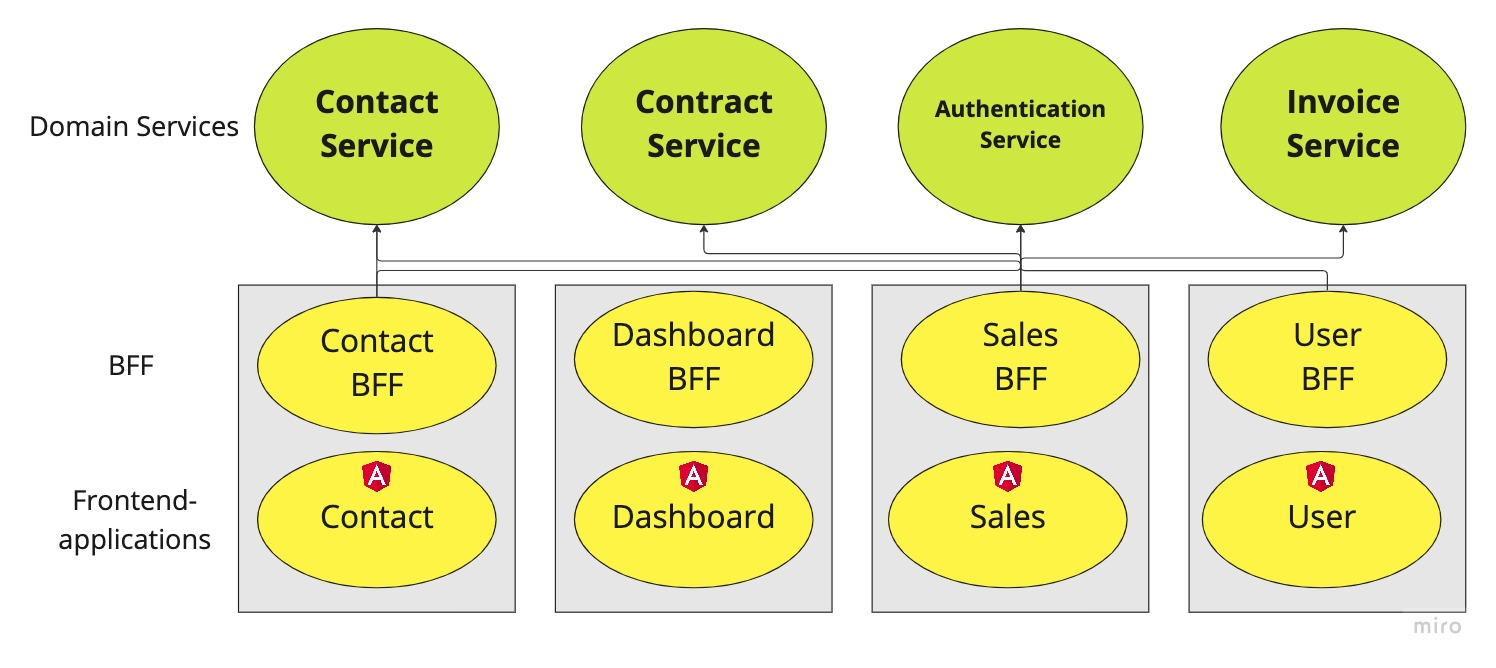
\includegraphics[width=0.8\linewidth]{images/ui-bff-architecture.jpg}
\caption{Frontend architecture with the backend-for-frontend pattern.}\label{figure:state-of-the-art:ui-bff-architecture}
\end{figure}
\fi

Figure \ref{figure:state-of-the-art:ui-bff-architecture} shows an exemplary micro-frontend architecture using the backend-for-frontend pattern. Each frontend has a service that retrieves data only for that specific client. Because the backend-for-frontends function as gateway to the domain services, the domain services can stay very generic and be reused by different clients. Backend-for-frontends should implement only the presentation logic that puts the data into the form that the client needs. It should avoid storing state. \cite{misc:2019:leitner:backend-for-frontends}

With this architectural approach the backend-for-frontend and the frontend form a single deployment unit. If one application is changed, the other needs needs to adapt the changes. GraphQL is a perfect technology for implementing a backend-for-frontend, because it is specifically designed for implementing the presentation-layer.

\subsection{GraphQL}

GraphQL was developed by Facebook and refers to itself as the query language for an API. It provides the client with the opportunity to ask exactly for the data is needed. GraphQL offers the advantage that all data must be loaded from only one URL. With the help of the types within the GraphQL schema, the technology offers an understandable description of the
API for clients. \cite{misc:-:graphql-org} The functionality of GraphQL on the frontend can be compared to SQL on the database level. The client writes its queries with the desired fields from a dataset.

\section{(technical) Motivation}

The motivation behind this project report is the creation of a micro-frontend prototype that should replace the old monolithic application within AGnet. The prototype should be more or less equal to the old applications in terms of functionality. The introduction of microservices in the company comes with other problems than a monolithic frontend. For example, all micro-frontends could potentially request the authenticated user. This leads to increased network traffic in comparison to a traditional frontend monotlith.

These problems should be researched and solved through using GraphQL. Many GraphQL clients provide some form of caching. Caching should be used to provide a single caching layer for all micro-frontends to avoid multiple requests to the same resource. GraphQL offers the possibility that the client directly writes the query to the backend. GraphQL provides the ability for the client to write the query directly to the backend. This opens the possibility of removing fields from GraphQL queries that are already in cache. These approaches to improving performance should be evaluated and compared to the naive approach without any optimizations.

\section{Hypothesis}

The first hypothesis focuses on the performance improvement that GraphQL can bring to micro-frontend architectures.

\paragraph{Hypothesis 1} 
A micro-frontend architecture using a shared GraphQL caching layer with partial data can solve the problems of over-fetching and over-requesting inside a distributed architecture. The total number of network-requests and network-traffic can be drastically reduced.\\\\

The second hypothesis focuses on the fact that the creation of a micro-frontend architecture should not depend on a single technology.

\paragraph{Hypothesis 2}
The micro-frontend architecture of the prototype provides enough freedom for an individual choice of technology.\\\\

The result of the work is the proof that GraphQL can solve problems of a micro-frontend architecture. The proof is provided through designing a micro-frontend architecture and writing a shared caching layer.
